\documentclass[12pt,a4paper,twoside]{article}
\usepackage[utf8]{inputenc}
\usepackage{amsmath}
\usepackage{lmodern}
\usepackage{textcomp}
\usepackage{amsfonts}
\usepackage{amssymb}
\usepackage{graphicx}
\usepackage[left=2cm,right=2cm,top=2cm,bottom=2cm]{geometry}
\author{Carlos Eduardo Martínez Núñez}
% used in maketitle                                                             
\title{\textbf{Movimiento de la Tierra Alrededor del Sol}}
\begin{document}
\maketitle
El presente estudio del movimiento de la tierra alrededor del sol, se centra en considerar el movimiento descrito por una trayectoria circular. Para tal fin se considera a la tierra discribiendo una circunferencia al rededor del sol con un radio medio de 1496000000 km, como muestra la gráfica 1. 
\begin{figure}[htbp]
\centering
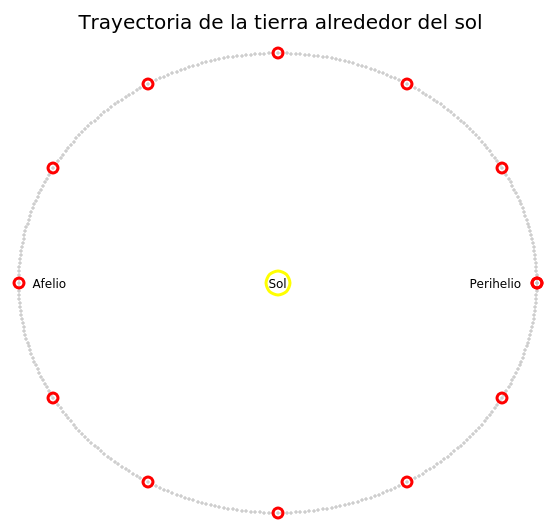
\includegraphics[width=12cm]{trtierra.png}
\caption{Trayectoria de la tierra alrededor del sol.}\label{fig:figura1}
\end{figure}
La trayectoria corresponde una una circunferencia descrita por la ecuación en coordenadas polares, dada como:
\begin{eqnarray}
r=1496000000
\end{eqnarray}
En termino de coordenadas cartesianas, esta trayectoria puede ser expresada por las ecuaciones:
\begin{eqnarray}
x=rcos(\theta)\\
y=rsin(\theta)
\end{eqnarray}
\section{Aplicación Fortran para el cálculo de la trayectoria de la la tierra alrededor del sol}
El código de la aplicación fortran para determinar la trayectoria en coordenadas cartesianas de la tierra alrededor del sol, corresponde a:
\begin{verbatim}
program mcircular
!::::::::::::::::::::::::::::::::::::::::::::::::::::::::::::::::::::::::::::::::::::
  !Aplicación Fortran para calcular la trayectoria y posiciones notables de la tierra
  !al rededor del sol
  !r------------radio medio de la tierra al sol
  !x------------Abcisa (coordenadas cartesianas)
  !y------------Ordenada (Coordenadas cartesianas)
  !f_x----------Función calculo de x
  !f_y----------Funición cálculo de y
  !a------------ángulo
!::::::::::::::::::::::::::::::::::::::::::::::::::::::::::::::::::::::::::::::::::::
  implicit none
  integer::i,j
  double precision, parameter::r=1.496d8, pi=3.141592d0
  double precision::a,f_x,f_y
  double precision,dimension(0:360)::x,y

  !Creando documento para almacenar datos
  open (1,file="tr_tierra.txt",status="unknown")
  !loop para el cálculo de la trayectoria
  do i=0,360
     !angulo en grados
     a=dble(i)
     a=a*pi/180.0d0
     !llamando funciones
     x(i)=f_x(a)
     y(i)=f_y(a)
     write (1,*) x(i),y(i), a
  end do
  close(1)
!:::::::::::::::::::::::::::::::::::::::::::::::::::::::::::::::::::::::::::::::::::
 !Creando segundo documento para las posiciones notables
 open (2,file="pst_tierra.txt",status="unknown")
 !loop para las posiciones notables 
  do j=0,360,30
     !angulo en grados
     a=dble(j)
     a=a*pi/180.0d0
     !llamando funciones
     x(j)=f_x(a)
     y(j)=f_y(a)
     write (2,*) x(j),y(j), a
  end do
  close(2)
end program mcircular 
!::::::::::::::::::::::::::::::::::::::::::::::::::::::::::::::::::::::::::::::::::

!Función para el cálculo de la abcisa (x)
function f_x(a)
implicit none
 !Función de conversión de coordenadas polares a cartesianas
  double precision, parameter::r=1.496d8
  double precision::f_x
  double precision, intent(in)::a
  f_x=r*dcos(a)
end function f_x
!:::::::::::::::::::::::::::::::::::::::::::::::::::::::::::::::::::::::::::::::::

!Función para el cálculo de la ordenada (y)
function f_y(a)
implicit none  
  !Función de conversión de coordenadas polares a cartesianas
  double precision, parameter::r=1.496d8
  double precision::f_y
  double precision, intent(in)::a
  f_y=r*dsin(a)
  end function f_y
\end{verbatim}
El Scritp para la graficación de los datos de salida usando Gnuplot corresponde a:
\begin{verbatim}
set title "Trayectoria de la tierra alrededor del sol"
set title font ",15" norotate
set style data lines
set style data points
set pointsize 0.5
unset key
unset border
unset xtics
unset ytics
set xrange [-150000000:150000000]
set yrange [-150000000:150000000]
set label 1 "Sol" at 0.0,0.0 center front
set label 2 "Perihelio" at 111600000.00000000, 0.0000000000000000
set label 3 "Afelio" at -141599999.99996805, 97.777033044205780
plot "tr_tierra.txt" using 1:2 ls 1 lw 1 lc rgb "gray",\
"pst_tierra.txt" using 1:2 ls 6 lw 10 lc rgb "red",\
"center.txt" using 1:2 ls 6 lw 24 lc rgb "yellow"
\end{verbatim}
\end{document}